% ART-MAPPO component-ablation insertion.
% Copy figures/art_mappo_component_ablation.pdf beside the manuscript or
% adjust the path below. Values are derived from the transferred CSV files.

\begin{figure*}[!t]
  \centering
  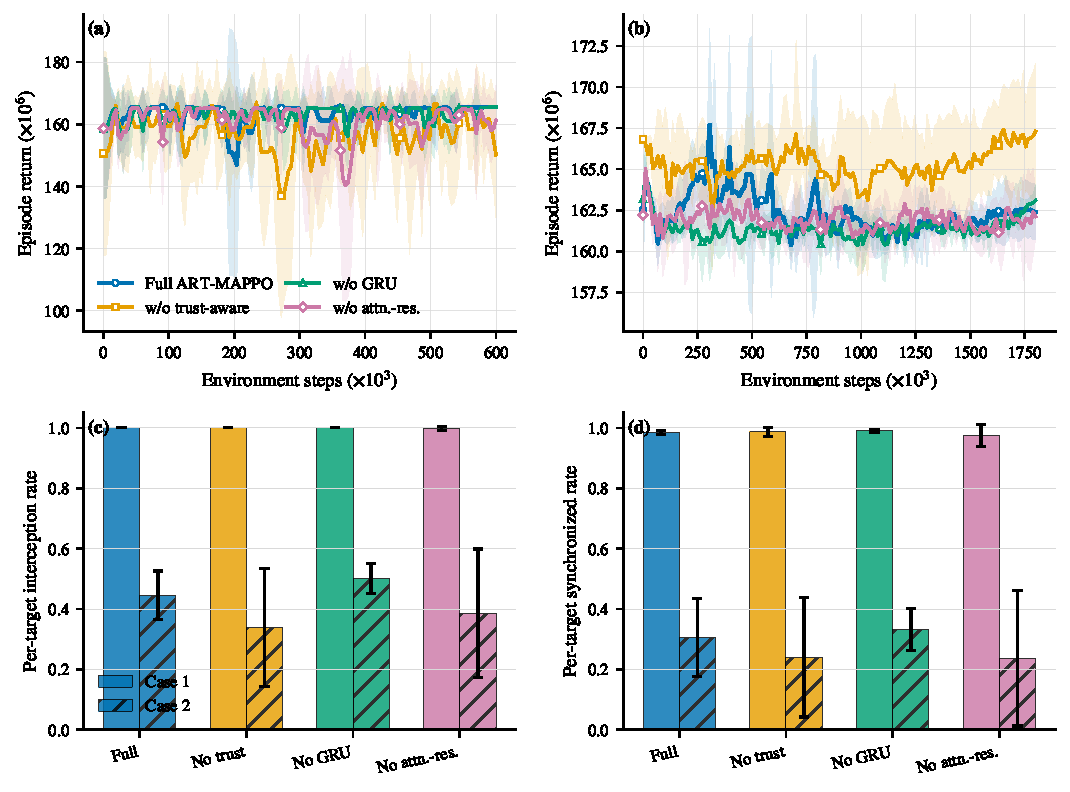
\includegraphics[width=\textwidth]{figures/art_mappo_component_ablation.pdf}
  \caption{Component ablation of ART-MAPPO over five paired training seeds.
  (a)--(b) Episode-return learning curves in Cases 1 and 2, respectively;
  solid lines and shaded regions denote the seed mean and 95\% confidence
  interval. (c)--(d) Held-out per-target interception and synchronized-
  interception rates over 20 common evaluation episodes per seed and case;
  error bars are 95\% Student-\(t\) confidence intervals over seed-level
  estimates. Trust-guided exploration is disabled during evaluation.}
  \label{fig:art_component_ablation}
\end{figure*}

\begin{table}[!t]
\centering
\caption{Pooled paired final-return ablation statistics}
\label{tab:art_component_ablation}
\setlength{\tabcolsep}{3.2pt}
\begin{tabular}{lrrrr}
\hline
Removed component &
$\Delta R$ ($10^6$) &
$d_z$ &
$p$ &
$p_{\mathrm{Holm}}$\\
\hline
Trust-aware & 0.697 & 0.102 & 0.7598 & 0.7598\\
GRU & 0.657 & 0.678 & 0.0645 & 0.1289\\
Attention--residual & 1.709 & 0.884 & 0.0156 & \textbf{0.0469}\\
\hline
\end{tabular}
\end{table}

\subsubsection{Component ablation}
To isolate the contribution of each architectural component, we compare full
ART-MAPPO with three single-component removals: trust-aware training, the GRU
temporal encoder, and the attention--residual backbone. All environment,
reward, optimizer, rollout-budget, target-assignment, and guidance settings
are held fixed. The MLP replacing the attention--residual backbone is
parameter matched. Each variant is trained with five paired seeds in both
cases (0.6 and 1.8 million environment steps for Cases 1 and 2), and every
trained seed is evaluated over 20 common held-out deterministic episodes,
yielding 800 episodes in total. Evaluation disables trust-guided exploration,
so the trust comparison measures its training-time effect.

Figure~\ref{fig:art_component_ablation} and
Table~\ref{tab:art_component_ablation} show that the
attention--residual backbone has the strongest independent evidence: removing
it reduces the pooled final return by $1.709\times10^6$ with a large paired
effect ($d_z=0.884$) and remains significant after Holm correction
($p_{\mathrm{Holm}}=0.0469$). In Case 2, the full model also exceeds this
ablation by 6.00 and 6.875 percentage points in per-target interception and
synchronized interception, respectively. The trust-aware mechanism yields
directional task-level gains in Case 2: the corresponding rates increase from
34.0\% to 44.625\% and from 24.0\% to 30.5\%. These pooled target-level
effects are not significant after correction, and are therefore not
overinterpreted. The full model has a positive pooled return difference over
the no-GRU variant ($d_z=0.678$), but the corrected test is not significant
and no-GRU is competitive on the Case-2 target metrics. Thus, the experiment
supports the backbone contribution, suggests a task-dependent trust benefit,
and indicates that the GRU advantage is conditional on the observation and
training regime.

For completeness, the stricter trial-level indicators are retained in the
reported data. Full ART-MAPPO attains 100\% all-target interception and 90\%
all-target synchronized interception in Case 1. In Case 2, the all-eight-
target indicator is zero for every variant at the present budget, creating a
floor effect; the figure therefore reports per-target rates while preserving
the strict metrics in the accompanying tables.
